\documentclass[10pt]{article}

\usepackage[a4paper,margin=21mm]{geometry}
\usepackage[utf8]{inputenc}
\usepackage[T1]{fontenc}
\usepackage{lmodern}
\usepackage[protrusion=true,expansion=false]{microtype}
\usepackage{graphicx}
\usepackage{booktabs}
\usepackage{tabularx}
\usepackage{array}
\usepackage{amsmath}
\usepackage{amssymb}
\usepackage{xcolor}
\usepackage{tikz}
\usetikzlibrary{arrows.meta,positioning,calc,fit,plotmarks}
\usepackage[numbers,sort&compress]{natbib}
\usepackage[hidelinks]{hyperref}
\usepackage{url}
\usepackage{caption}
\usepackage{fancyhdr}
\usepackage{float}

\definecolor{mqnavy}{HTML}{173F6D}
\definecolor{mqblue}{HTML}{2C6EAA}
\definecolor{mqteal}{HTML}{287D78}
\definecolor{mqgreen}{HTML}{2E7D32}
\definecolor{mqorange}{HTML}{C46A14}
\definecolor{mqred}{HTML}{B23A2B}
\definecolor{mqgray}{HTML}{66727D}
\definecolor{mqgrid}{HTML}{D9E0E6}
\definecolor{mqlightblue}{HTML}{EAF1F8}
\definecolor{mqpaleblue}{HTML}{EDF5FB}
\definecolor{mqpaleteal}{HTML}{ECF7F6}
\definecolor{mqpalegreen}{HTML}{EFF8F0}
\definecolor{mqpaleorange}{HTML}{FFF6EA}
\definecolor{mqpalered}{HTML}{FCEFED}

\hypersetup{
  pdftitle={HPC-MQBench: Qualification-First Benchmarking on Slurm - Design and Evaluation with Apache Kafka},
  pdfauthor={Sepehr Mahmoodian and Julian Kunkel},
  pdfsubject={Qualification-first distributed messaging benchmarking on Slurm-managed HPC systems},
  pdfkeywords={distributed messaging, benchmark methodology, Slurm, HPC, qualification, Kafka, performance evaluation}
}

\captionsetup{font=small,labelfont=bf,justification=raggedright,singlelinecheck=false}
\renewcommand{\arraystretch}{1.12}
\newcolumntype{Y}{>{\raggedright\arraybackslash}X}
\newcolumntype{L}[1]{>{\raggedright\arraybackslash}p{#1}}
\newcommand{\system}{HPC-MQBench}
\newcommand{\qualified}{\textsc{Qualified}}
\newcommand{\overdriven}{\textsc{Overdriven}}
\newcommand{\ineligible}{\textsc{Ineligible}}
\setlength{\emergencystretch}{2em}
\makeatletter
\setlength{\@fptop}{0pt}
\setlength{\@fpsep}{14pt}
\setlength{\@fpbot}{0pt plus 1fil}
\makeatother

\pagestyle{fancy}
\fancyhf{}
\lhead{\system}
\rhead{Qualification-first messaging benchmarking}
\cfoot{\thepage}
\setlength{\headheight}{14pt}

\title{\textbf{HPC-MQBench: Qualification-First Benchmarking on Slurm}\\[0.4em]\large Design and Evaluation with Apache Kafka}
\author{Sepehr Mahmoodian, Julian Kunkel}
\date{}

\begin{document}
\maketitle

\begin{abstract}
Benchmarking a messaging system on an HPC cluster requires coordinated service
startup, client placement, measurement, and recovery within scheduler allocations.
We present \system{}, a Slurm-native benchmark that handles this workflow and
checks record envelopes, delivery accounting, and delivery pressure before ranking endpoint rates.
We evaluate a single Kafka broker with RAM-backed logs using 120 workload
configurations, broker-profile screening, and two five-block validation stages.
Screening yields 99 qualified cases, 14 outside the producer-delivery policy,
and seven with invalid evidence.  Within the retained V2 stage, the procedure
ranks \texttt{cfg\_007} first: five qualified observations, with medians of
2,927 MiB/s balanced endpoint rate, 1.24\% pending deliveries, and 2.56 s p99 latency.
It qualifies in only two of five V1 observations, and V1 qualification changes
at an allocation boundary.  This is a stage-specific selection, not a stable
configuration recommendation.  The short-window results demonstrate policy-based
selection and the importance of allocation context; monitoring does not identify
a unique bottleneck.  Retained summaries support auditing the decisions, but
missing campaign provenance prevents full reconstruction.
\end{abstract}

\noindent\textbf{Keywords:} HPC; Slurm; Kafka; messaging benchmarks; traceability

\section{Introduction}
\label{sec:introduction}

Scientific instruments, telemetry services, and simulations produce streams that
must reach downstream analysis without tightly coupling every producer to every
consumer.  Messaging systems provide this separation in neutron-instrument
pipelines and HPC telemetry services~\cite{mukai2018ess,adamson2023stream}.
Choosing a configuration requires more than finding the highest producer rate:
records may still await delivery, consumers may fall behind, or latency may become
unacceptable.  Tail-latency studies show why occasional slow responses matter
even when typical response times are low~\cite{dean2013tail}.

HPC adds an execution problem.  Services and clients must start on allocated
nodes, finish within job limits, and leave enough evidence to recover from an
interruption.  A messaging experiment therefore needs an explicit connection
between scheduler state, measurement validity, and configuration selection.
\system{} brings those operations into a single Slurm workflow.
It records placement and settings, measures both endpoints, checks record
envelopes and delivery counts, and separates invalid runs from completed runs
that exceed a declared delivery
policy.  Qualification takes precedence over endpoint rate in the campaign ranking.

This paper presents the benchmark design and evaluates Kafka with it.  The
contributions are: (1) a scheduler-managed experiment lifecycle with resumable
state and recorded inputs; (2) an explicit measurement contract and delivery policy that keep
endpoint rates, correctness, latency, and pending deliveries distinct; and (3) a Kafka
evaluation covering parameter screening, repeated validation, and resource-based
analysis of where performance may be limited.

\section{Related Work}
\label{sec:related-work}

Kafka's original design combines partitioned logs, batching, and pull-based
consumption~\cite{kreps2011kafka}.  Empirical studies examine ingestion limits,
client settings, and deployment choices~\cite{hesse2020kafka,fu2021fair};
comparative work also considers the delivery guarantees behind performance
results~\cite{dobbelaere2017kafka}.

OpenMessaging Benchmark supplies workloads and messaging drivers, while
SPECjms2007 defines validity and disclosure rules for JMS
experiments~\cite{openmessagingbenchmark,specjms2007}.  Stream-processing
benchmarks such as Linear Road examine continuous queries, and later work
addresses workload and latency measurement~\cite{arasu2004linearroad,karimov2018streambench}.
RIoTBench supplies IoT microbenchmarks and application workloads, while ESPBench
combines enterprise workloads with result validation and latency
measurement~\cite{shukla2017riotbench,hesse2021espbench}.  These stream-processing
benchmarks assess application workloads; \system{} focuses on messaging
delivery and experiment control within Slurm allocations.

Scientific streaming already has HPC implementations.  Pilot-Streaming manages
stream-processing frameworks on HPC resources; Mofka provides an event-streaming
system designed for supercomputers~\cite{chantzialexiou2018pilotstreaming,dorier2025mofka}.
ADIOS~2 provides a broader scientific data-management framework with file and
memory-based data movement~\cite{godoy2020adios2}.
ReFrame and Popper address scheduled testing and executable
provenance~\cite{karakasis2020reframe,jimenez2017popper}.
Work on measurement bias and statistical benchmarking motivates recording
experimental context and reporting variation across
runs~\cite{mytkowicz2009wrongdata,kalibera2013rigorous,hoefler2015scientific}.
Validity rules and workload generators are established ideas.  Our contribution
is the enforced connection between experiment state and messaging evidence
(Table~\ref{tab:related-comparison}).  A completed Slurm job alone is insufficient:
resume checks verify saved inputs and outputs, measurement checks determine case
eligibility, and delivery policy determines which eligible cases enter the
qualified ranking.  Implementing this with another harness would require the
same messaging-specific checks and state transitions.  We demonstrate this
integration; we claim neither that its components are new nor that competing
harnesses cannot implement it, and we do not compare harness efficiency.

\begin{table}[!htbp]
\centering
\footnotesize
\begin{tabularx}{\linewidth}{@{}L{0.18\linewidth}Y Y@{}}
\toprule
System & Execution and recovery & Evidence and decisions \\
\midrule
OpenMessaging Benchmark~\cite{openmessagingbenchmark} & Base framework: messaging-driver interface and distributed workload workers. & Publish/consume rates, errors, latency distributions, and sent-minus-received backlog adjusted for subscriptions. \\
ReFrame~\cite{karakasis2020reframe,reframedocs} & Scheduler-backed test pipeline, job monitoring, and cleanup. & User-defined sanity checks and performance references; retained test results. \\
SPECjms2007~\cite{specjms2007} & Prescribed JMS workload and system-under-test rules. & Clock, steady-state, message-count and latency validity rules; full disclosure. \\
\system{} & Slurm role placement; adapter-specific restart/cleanup (per-case Kafka restart and log reset here); input/output checks before checkpoint reuse. & Endpoint accounting, envelopes and offset checks, clock-gated latency, qualification before ranking, manifests and machine-readable decisions. \\
\bottomrule
\end{tabularx}
\caption{Documented scope of related tools and this implementation. This compares
their supplied abstractions, not every possible extension or an experimentally
measured advantage. OpenMessaging's backlog is a message-count difference, not
the producer-callback pending ratio used here.}
\label{tab:related-comparison}
\end{table}

\section{Benchmark Design}
\label{sec:architecture}

Sections~\ref{sec:architecture}--\ref{sec:measurement} describe the inspected
implementation and the retained measurement contract.  The original campaign
source snapshot is unavailable; Section~\ref{sec:threats} distinguishes what
the retained results establish from what the current code implements.

\subsection{Placement and software components}

The evaluated deployment uses four exclusive nodes: producer/controller,
Kafka broker, consumer, and monitoring/results (Figure~\ref{fig:system-architecture}).
MPI rank 0 coordinates the workers through \texttt{mpi4py}~\cite{dalcin2021mpi4py};
each active producer or consumer rank owns a Kafka client.
Prometheus collects Kafka/JVM metrics from the JMX Exporter Java
agent~\cite{prometheus,kafkamonitoring}.  The scripts also enable
\texttt{node\_exporter} for host metrics and \texttt{kafka\_exporter} for Kafka
metadata and consumer-group lag where available.  The paper's pending-delivery
ratio comes from producer callbacks.  A separate Python monitor reads
Linux procfs for broker CPU/RSS, sysfs for interface byte counters, and
\texttt{statvfs} for tmpfs occupancy.  The campaign scripts configure one-second
process sampling, Prometheus scrapes, and range-query steps.

\begin{figure}[H]
\centering
\resizebox{0.97\linewidth}{!}{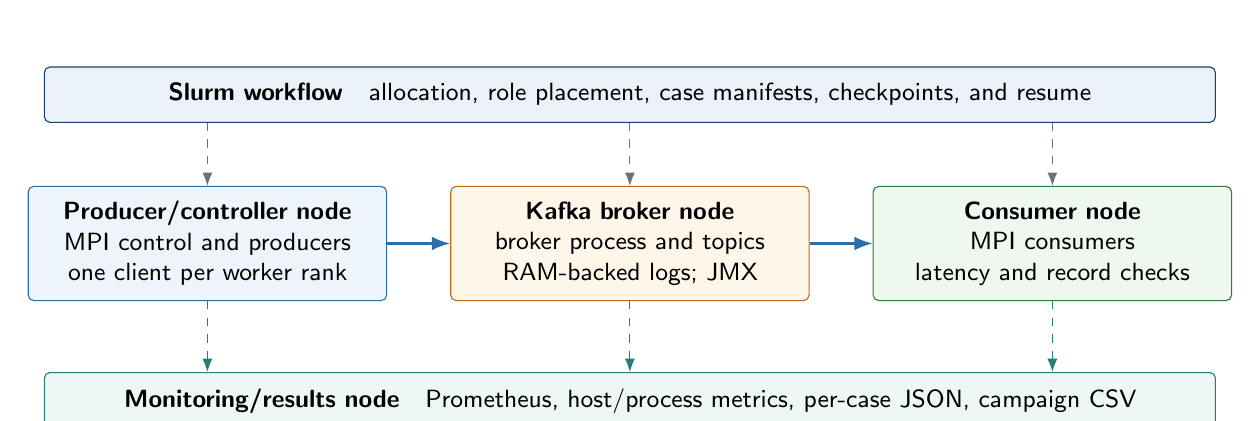
\begin{tikzpicture}[
 >=Latex, font=\sffamily\small,
 box/.style={draw,rounded corners=2pt,text width=4.2cm,minimum height=1.45cm,align=center,inner sep=5pt},
 band/.style={draw=mqnavy,fill=mqlightblue,rounded corners=2pt,text width=14.45cm,align=center,inner sep=6pt}
]
\node[band] (control) {\textbf{Slurm workflow}\quad allocation, role placement, case manifests, checkpoints, and resume};
\node[box,draw=mqorange,fill=mqpaleorange,below=8mm of control] (broker)
 {\textbf{Kafka broker node}\\broker process and topics\\RAM-backed logs; JMX};
\node[box,draw=mqblue,fill=mqpaleblue,left=8mm of broker] (producer)
 {\textbf{Producer/controller node}\\MPI control and producers\\one client per worker rank};
\node[box,draw=mqgreen,fill=mqpalegreen,right=8mm of broker] (consumer)
 {\textbf{Consumer node}\\MPI consumers\\latency and record checks};
\node[band,draw=mqteal,fill=mqpaleteal,below=9mm of broker] (monitor)
 {\textbf{Monitoring/results node}\quad Prometheus, host/process metrics, per-case JSON, campaign CSV};
\draw[->,thick,mqblue] (producer.east) -- (broker.west);
\draw[->,thick,mqblue] (broker.east) -- (consumer.west);
\foreach \n in {producer,broker,consumer} {
 \draw[->,dashed,mqgray] (control.south -| \n.north) -- (\n.north);
 \draw[->,dashed,mqteal] (\n.south) -- (monitor.north -| \n.south);
}
\end{tikzpicture}
}
\caption{Four-node Kafka deployment.  Solid arrows carry records; dashed lines
show control and monitoring.  Exporters run beside the resources they observe.}
\label{fig:system-architecture}
\end{figure}

The common benchmark code owns workload timing, record identity, result schemas,
and qualification.  The Kafka adapter supplies \texttt{confluent-kafka}/librdkafka
clients, starts and stops the broker, creates topics, and records effective client
and broker settings.  This interface keeps product-specific operations separate
from experiment control.  Additional adapters can use the same interface; the
measurements in this paper are from Kafka.

\subsection{Campaign execution and recovery}

\textbf{V1} denotes the initial workload campaign: 120 screening configurations
under baseline broker profile B0, followed by five-block validation of ten
shortlisted workloads.  \textbf{V2} denotes the subsequent instrumentation check,
latency-load calibration, broker-profile screening and confirmation, and
five-block final validation.  These are campaign labels, not Kafka versions.
V2 retained B0 and repeated the same ten workloads in this evaluation.

The workflow validates the environment and case manifests, requests Slurm
allocations, places roles with job steps, and runs cases sequentially within each
batch~\cite{jette2003slurm}.  Independent screening batches can execute in parallel.
The Kafka campaign runner restarts Kafka and clears the configured RAM-backed
log storage before each case.  Each stage records job IDs, settings, timestamps, result paths, and
checksums.  A resumed campaign reuses a completed stage only after its inputs and
output files pass these checks.  Missing files or changed inputs stop reuse.
A scheduler failure is recorded as a workflow failure, separate from a completed
benchmark case with invalid measurements.

\subsection{Automated analysis and retained outputs}
\label{sec:analysis-outputs}

The workflow analyzes results as each campaign stage finishes
(Figure~\ref{fig:analysis-outputs}).  It checks case completeness and measurement
validity, calculates endpoint and balanced rates, and classifies delivery
pressure using pending deliveries, flush time, and failed sends.  Screening produces a
ranked table and a validation shortlist.  Repeated validation reports eligible
and qualified counts, balanced endpoint-rate medians and variability, pending deliveries, and latency.
Validation summaries use eligible observations, including overdriven ones;
qualified-observation count takes priority in the final ranking.

Kafka profile analysis summarizes process and JMX samples from the producer
measurement interval:
CPU, memory, tmpfs occupancy, traffic, request queues and timing, and garbage
collection.  It records instrumentation, profile-screening, and confirmation
decisions (Section~\ref{sec:profile-selection}).  Per-case reports contain threshold-based diagnostic flags for
delivery pressure and resource use.  These flags guide inspection; identifying
a bottleneck still requires checking measurement coverage, timing, and scope.

Each completed case writes \texttt{final\_report.json}, available monitoring data, and an
event timeline.  The completed V1 and V2 bundles contain screening rows,
validation observations, and ranked summaries in CSV and JSON; a campaign-level JSON
report records the recommendation.  Resource summaries and broker-profile
decisions remain in the stage-analysis directories.  Source-report paths and
hashes link summaries to individual cases.  The workflow also saves configuration
manifests, job IDs, software/provenance records, checkpoints, and checksums.
Section~\ref{sec:threats} identifies gaps in the retained campaign provenance.
Latency outputs contain histograms and summaries, not individual-message traces.
The full workflow selects machine report mode; standalone cases can additionally
produce Markdown, HTML, and plots in presentation modes.
The parameter contrasts, threshold sensitivity, and block-level comparisons in
this paper are downstream analyses of the retained campaign data.

% Source: report_builder.py; analyze_kafka_reproducible_campaign.py;
% analyze_broker_tuning_v2.py; finalize_reproducible_results.py;
% workflow/engine.py.
\begin{figure}[!htbp]
\centering
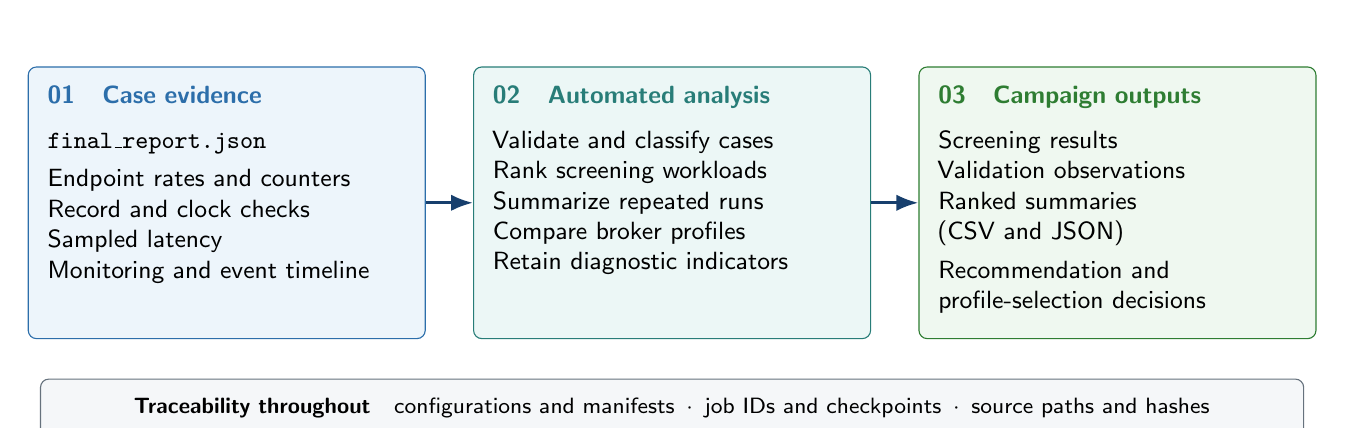
\begin{tikzpicture}[
 >=Latex,font=\sffamily\small,
 card/.style={draw,rounded corners=3pt,text width=4.55cm,
   minimum height=3.45cm,align=left,inner sep=7pt},
 support/.style={rounded corners=3pt,text width=15.55cm,align=center,
   inner sep=7pt,font=\sffamily\footnotesize},
 flow/.style={->,line width=1.1pt,mqnavy}
]
\node[card,draw=mqblue,fill=mqpaleblue] (evidence) {
 \begin{minipage}[t][2.95cm][t]{4.55cm}
 {\color{mqblue}\textbf{01\quad Case evidence}}\\[5pt]
 \texttt{final\_report.json}\\[3pt]
 Endpoint rates and counters\\
 Record and clock checks\\
 Sampled latency\\
 Monitoring and event timeline
 \end{minipage}};
\node[card,draw=mqteal,fill=mqpaleteal,right=6mm of evidence] (analysis) {
 \begin{minipage}[t][2.95cm][t]{4.55cm}
 {\color{mqteal}\textbf{02\quad Automated analysis}}\\[5pt]
 Validate and classify cases\\
 Rank screening workloads\\
 Summarize repeated runs\\
 Compare broker profiles\\
 Retain diagnostic indicators
 \end{minipage}};
\node[card,draw=mqgreen,fill=mqpalegreen,right=6mm of analysis] (outputs) {
 \begin{minipage}[t][2.95cm][t]{4.55cm}
 {\color{mqgreen}\textbf{03\quad Campaign outputs}}\\[5pt]
 Screening results\\
 Validation observations\\
 Ranked summaries\\
 {\small (CSV and JSON)}\\[3pt]
 Recommendation and\\
 profile-selection decisions
 \end{minipage}};
\draw[flow] (evidence.east) -- (analysis.west);
\draw[flow] (analysis.east) -- (outputs.west);
\node[support,draw=mqgray,fill=mqgrid!25,below=5mm of analysis] (audit) {
 \textbf{Traceability throughout}\quad
 configurations and manifests\enspace $\cdot$\enspace job IDs and checkpoints\enspace
 $\cdot$\enspace source paths and hashes};
\end{tikzpicture}
\caption{Outputs of a completed Kafka campaign.  The workflow generates the
case evidence, analysis, and machine-readable result bundles automatically.
Screening and validation tables are saved in both CSV and JSON; recommendation
and profile-selection decisions are recorded in JSON.}
\label{fig:analysis-outputs}
\end{figure}

\section{Measurement and Qualification}
\label{sec:measurement}
\label{sec:qualification}

\subsection{Timing, records, and latency}

The evaluated profile uses a 15 s warm-up and a 30 s measurement window.
These campaign settings describe short-window performance; no duration-sensitivity
experiment establishes steady state.
At measurement end,
producers stop submitting records and count unresolved delivery callbacks before
flushing.  In librdkafka, delivery callbacks report success or failure to the
application~\cite{librdkafkaintroduction}.  Consumers keep polling during flush, then drain for up to 60 s to
account for callback-confirmed measurement records
(Figure~\ref{fig:qualification-workflow}).  Warm-up records are excluded.

\begin{figure}[!htbp]
\centering
\resizebox{\linewidth}{!}{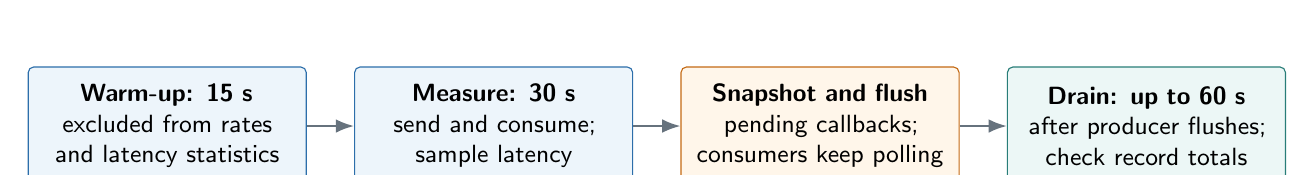
\begin{tikzpicture}[
 >=Latex,font=\sffamily\small,
 phase/.style={draw=mqblue,fill=mqpaleblue,rounded corners=2pt,text width=3.25cm,minimum height=1.5cm,align=center,inner sep=4pt}
]
\node[phase] (warmup) {\textbf{Warm-up: 15 s}\\excluded from rates\\and latency statistics};
\node[phase,right=6mm of warmup] (measure) {\textbf{Measure: 30 s}\\send and consume;\\sample latency};
\node[phase,draw=mqorange,fill=mqpaleorange,right=6mm of measure] (flush)
 {\textbf{Snapshot and flush}\\pending callbacks;\\consumers keep polling};
\node[phase,draw=mqteal,fill=mqpaleteal,right=6mm of flush] (drain)
 {\textbf{Drain: up to 60 s}\\after producer flushes;\\check record totals};
\foreach \a/\b in {warmup/measure,measure/flush,flush/drain}
 \draw[->,thick,mqgray] (\a.east) -- (\b.west);
\end{tikzpicture}
}
\caption{Case timing.  Pending deliveries are counted before flush; record
accounting continues through the bounded drain.}
\label{fig:qualification-workflow}
\end{figure}

Every record carries a 32-byte binary envelope containing producer identity,
sequence, flags, and a checksum of the envelope metadata.  Consumers validate
envelopes, check for repeated or regressing topic-partition offsets within each
consumer, and compare total consumption through drain with producer-confirmed
deliveries to detect missing or surplus counts.
Every tenth measurement record carries a timestamp taken after payload
generation, immediately before envelope encoding and submission.  The consumer
timestamps reception after polling and envelope/offset checks.  Latency therefore
includes client buffering and consumer polling, and covers sampled deliveries
through flush and drain; it excludes payload generation and waiting in the rate
scheduler.  The consumer rate counts only arrivals by its measurement deadline.

Before and after each case, 100 MPI ping-pong exchanges per worker estimate its
offset from rank~0.  The minimum-round-trip sample supplies the midpoint offset
and half-round-trip uncertainty estimate; the initial offset is used throughout
the run.  Validity requires every active rank's estimated uncertainty and offset
change to be at most 250 microseconds, no negative latency, and a nonzero observed
sample count equal to producer-confirmed sampled deliveries.  These gates do not
guarantee 250-microsecond end-to-end accuracy.

Each consumer accumulates a histogram with upper bounds spaced by
1~$\mu$s up to 1~ms, 10~$\mu$s from 1--10~ms, 100~$\mu$s from 10--100~ms,
1~ms from 100~ms--1~s, 10~ms from 1--10~s, and 100~ms from 10--60~s.
Each nonnegative sample enters the first bucket whose upper bound is at least
its latency.  Corresponding bucket counts are summed across consumer ranks.
For percentile $p$ and $N$ pooled samples, the estimate is the first bucket
upper bound whose cumulative count reaches $\lceil pN/100\rceil$, without
interpolation.  Samples above 60~s contribute to $N$; a percentile falling
in this overflow region uses the observed maximum.  The recorded 19.5~ms
p99 for \texttt{cfg\_090} is consistent with the 100~$\mu$s grid: it is the
upper edge of the $(19.4,19.5]$~ms bucket.  Its original histogram is unavailable
for independent recounting.  Validation summaries take medians of per-run
percentiles rather than pooling samples across runs.

The workload uses fixed-size synthetic payloads derived from JSON templates
with round-robin source IDs.  The envelope replaces the first 32 bytes,
preserving the configured record size.
Each producer rank has 50,000 IDs, so the screen covers 0.8--3.2 million configured
logical sources.  These IDs share a rank's client and rate controller; they are
not independent device connections.  Sampling every tenth sequence selects the
same tenth of these round-robin IDs; latency representativeness across sources
is unverified.  Source IDs are record keys; consumer
ranks share one case-specific group and divide the topic partitions.  The
maximum-load generator submits as fast as payload construction, client calls,
and callback polling permit; it does not impose an independent arrival stream.

\subsection{Endpoint rates and pending deliveries}

Let $B_p$ be bytes from measurement-period sends whose delivery is confirmed,
including confirmations during flush.  Let $B_c$ count measurement-tagged
record bytes received by the consumer measurement deadline.  Both counters
are summed across ranks.  Producer duration $T_p$ is the maximum recorded rank duration
from measurement start through flush completion.  Consumer duration $T_c$ is the
maximum recorded measurement duration, excluding drain.  Rates in MiB/s are
\begin{equation}
 R_p=\frac{B_p}{T_p2^{20}},\qquad
 R_c=\frac{B_c}{T_c2^{20}},\qquad
 R_{\mathrm{bal}}=\min(R_p,R_c).
 \label{eq:balanced-throughput}
\end{equation}
For fixed payload size $S$ bytes, the corresponding balanced record rate is
$R_{\mathrm{records}}=R_{\mathrm{bal}}2^{20}/S$.
Byte rates count record values, including the envelope, and exclude record keys
and protocol overhead.  We call $R_{\mathrm{bal}}$ the \emph{balanced endpoint rate}.
Using the minimum prevents a faster endpoint alone from raising the ranking
score; it is a conservative summary of the two reported rates.  Their windows
differ, so it is not a synchronized end-to-end steady-state throughput estimate,
and their ratio is not consumer lag.  The retained summaries cannot recover a
common-window delivered rate or consumer-progress trajectory.

We count unresolved producer delivery callbacks at flush start.
We express pending deliveries and failed sends as numeric
percentage values (for example, 5 denotes 5\%):
\begin{equation}
 D_{\mathrm{pending}}=100\frac{N_{\mathrm{pending}}}{N_{\mathrm{attempts}}},
 \qquad
 F_{\mathrm{send}}=100\frac{N_{\mathrm{failed}}}{N_{\mathrm{attempts}}}.
 \label{eq:pending-delivery}
\end{equation}
Here $N_{\mathrm{attempts}}$ includes every measurement-period send attempt,
and $N_{\mathrm{failed}}$ includes immediate submission errors and failed delivery
callbacks.  All counts are summed across producer ranks.  For each rank, pending
callbacks equal enqueued measurement records minus observed measurement delivery
callbacks, clamped at zero.  The CSV stores
$D_{\mathrm{pending}}$ under the legacy field name \texttt{pending\_backlog\_percent}.
This ratio measures producer-side delivery pressure, not broker queue depth or consumer
lag.  Broker queues are reported separately in the resource analysis.

\subsection{Validity before performance ranking}

A case is \ineligible{} if it fails execution, measurement-contract, backend-health,
latency, or record checks.  An eligible case is \qualified{}
under \texttt{qualification.application.v1} when
\begin{equation}
 D_{\mathrm{pending}}\leq5,\qquad
 T_{\mathrm{flush}}\leq10\ \mathrm{s},\qquad
 F_{\mathrm{send}}\leq0.1.
 \label{eq:qualification-policy}
\end{equation}
The first and third limits therefore mean 5\% and 0.1\%, respectively.
$T_{\mathrm{flush}}$ is the maximum rank-level flush duration, measured
from send-loop end to flush completion; the producer flush timeout is 30~s.
An eligible case exceeding any limit is \overdriven{}.  We treat the retained
thresholds as an illustrative policy: no recorded application requirement
justifies these particular values.  They are neither Kafka capacity limits nor
a validated service-level objective.  Qualification imposes no latency target
and does not prove steady state.  Record accounting uses confirmed deliveries,
so a permitted failed send is not a missing delivered record.  The inspected
send loop counts immediate submission failures and advances to the next record;
it does not resubmit the failed record at application level.  A strict-delivery
application would need a zero-failure policy and an explicit latency objective.

Repeated validation runs each shortlisted configuration once in each of five
randomized blocks.  Ranking first uses the number of qualified observations, then
median balanced endpoint rate.  Its interquartile range (IQR), pending
deliveries, flush, failures, and configuration ID resolve further ties.  This
reduces the influence of an unusually fast run.  IQR uses inclusive quartiles;
with five observations it is the fourth minus the second ordered value.  Qualification
counts and medians are descriptive, not estimates of a guaranteed success rate
or tests of statistical superiority.
The secondary rate statistic describes all eligible observations, retaining
overdriven cases rather than conditioning that summary on passing the policy.
This is the implemented rule, not a claim that it is optimal: at equal qualified
counts, overdriven rates can affect the order. Section~\ref{sec:profile-selection}
checks the alternative of using only qualified observations for that median.

\section{Experimental Setup}
\label{sec:experimental-setup}
\label{sec:audit}

The campaign ran on GWDG's \texttt{standard96s} partition using exclusive
four-node allocations and a two-hour job limit. The published node specification
lists 96 physical CPU cores, 514,000 MB RAM, and a 100 Gbit/s Omni-Path
fabric~\cite{gwdgcpupartitions}. Appendix~\ref{app:configuration} collects the
hardware specifications, recorded runtimes, workload settings, and broker profiles.
Published specifications provide context; the retained campaign lacks a complete
per-node snapshot, active SMT settings, CPU binding, and measured CPU frequencies.


The deployment used one KRaft broker, replication factor one, leader
acknowledgements (\texttt{acks=1}), no compression, and RAM-backed logs.
Workload screening and repeated validation use maximum offered load, with
producers and consumers running simultaneously under baseline broker profile B0.

The batch runner uses \texttt{iperf3}~\cite{iperf3} to probe TCP throughput before
Kafka starts, once per allocation: first producer to broker, then broker to
consumer.  The inspected collector defaults to ten seconds and four parallel
streams (\texttt{-t 10 -P 4 -J}); these are code defaults because the original
probe settings and raw JSON were not retained.  The analysis preserves
directional summaries, shared by cases in each batch.  This TCP test is not an
RDMA benchmark or a measurement of nominal fabric speed.  The inventory code
also queries \texttt{lscpu}, \texttt{numactl}, procfs, sysfs/\texttt{ethtool}, and
a repository-local, single-process STREAM-style memory probe.  The missing raw
inventory prevents using those probes as measured hardware or memory-bandwidth
results here.

Appendix Table~\ref{tab:parameter-space} gives the baseline and every screened parameter
level.  The 120 unique configurations comprise one baseline, 43 one-factor contrasts,
nine additional producer/consumer rank pairs, and 67 mixed configurations sampled
with seed 42 after duplicate removal.  Four Slurm jobs each run up to 30 cases.
The one-factor cases hold the other ten settings at baseline.  The mixed cases
extend coverage without forming a full factorial design.


The ten-workload shortlist combines the three highest-ranked qualified cases,
the overdriven case nearest the pending-delivery limit that passes the other delivery
limits, the highest-rate overdriven case, the eligible byte-rate and
record-rate leaders, the baseline, and the strongest one-factor case.  After
deduplication, qualification-ranked cases fill the list to ten for V1 and V2.
The inspected generators use Python's \texttt{random.Random(20260728)} and
\texttt{shuffle}: one generator per stage advances across blocks, each of which
shuffles a fresh copy of the shortlist. Replaying this procedure reproduces all
five manifest orders;
V1 and V2 use identical orders. The companion supplement lists every validation
case's block, order, and batch, alongside the available allocation IDs; V2 retains
stage-level job IDs without an explicit case-to-job mapping. Its retained
report paths contain \texttt{batch\_001} for blocks 1--3 and \texttt{batch\_002}
for blocks 4--5, establishing batch membership independently of the missing job mapping.

This was an exploratory campaign with recorded operational changes.  Two repairs
of \texttt{cfg\_103} remained invalid; the selected screen contains 119 original
observations and its last repair.  The controller was allowed to complete the
stage with seven invalid cases, all excluded from performance selection under
unchanged per-case rules.  The retained workflow history records the repairs
and input canonicalization; raw results were unchanged.

We audited all 220 selected screening and repeated-validation rows, with no
mismatch in the recomputable quantities (Table~\ref{tab:auditability}).
The execution history contains 120 original screening runs, two repair runs,
100 validation runs, and 69 V2 instrumentation, calibration, and broker-profile
runs: 291 executions in total.  The 69 comprise six instrumentation runs,
three calibration runs, 30 profile-screening runs, and 30 additional confirmation
runs.  The 220-row audit uses one selected observation per screening
configuration and all 100 validation observations; it excludes the original
\texttt{cfg\_103} observation and its superseded repair.
Separate source tests cover policy boundaries, malformed records, ordering,
invalid latency, health failures, and resume checks. The local companion folder
retains case rows, supporting summaries, and verification scripts; it is not a
complete raw campaign archive.

\begin{table}[H]
\centering
\footnotesize
\begin{tabularx}{\linewidth}{@{}L{0.23\linewidth}Y@{}}
\toprule
Evidence level & What can be checked \\
\midrule
Recomputed from case rows & Endpoint minima, record-rate conversions, pending and failed-send ratios, classifications from retained validity flags/counters, summaries across observations, and allocation-aligned block counts. \\
Retained summaries & Endpoint rates, per-run latency percentiles, clock-validity flags, and monitoring aggregates. Raw per-rank times, histograms, clock exchanges, and traces are unavailable for independent reconstruction. \\
Inspected current code & Timing and histogram algorithms, probe parsing, qualification and resume logic; source tests establish current behavior, not campaign-time code identity. \\
Unrecovered context & Campaign commit, exact Kafka/client versions, node inventory and binding, raw network probes, and negotiated routes/link rates. \\
\bottomrule
\end{tabularx}
\caption{Auditability of the retained study. Agreement with an estimator or a
summary is distinguished from reconstruction of its original measurements.}
\label{tab:auditability}
\end{table}

% Sources: data/kafka/derived/{phase1_configuration_outcomes,backlog_sensitivity,
% workload_regimes,spearman_correlations}.csv; data/kafka/source/artifacts/
% {v1,v2}/validation_repeats.csv; data/kafka/source/artifacts/v2/validation_summary.csv;
% data/kafka/source/analysis/v2/profile-confirmation/kafka_broker_tuning_v2_decisions.json.
\section{Kafka Performance Evaluation}
\label{sec:kafka-evaluation}

We evaluate short-window Kafka performance through screening, repeated validation,
and broker-profile selection. The questions are the balanced endpoint rate under the
stated policy, where pending deliveries and latency grow, and which screening
results survive repetition. The setup and baseline settings are given in
Section~\ref{sec:experimental-setup}.

\subsection{Screening results under the delivery policy}

Of the 120 selected screening observations, 113 are eligible and 99 are qualified.
Seven fail the latency-validity checks; one of these also reports 83,350
unexplained surplus records. These observations remain in the evidence but are
excluded from performance selection. Figure~\ref{fig:kafka-operating-limits}
shows balanced endpoint rate and latency against the producer pending-delivery ratio
defined in Equation~\eqref{eq:pending-delivery}.

\begin{figure}[!htbp]
\centering
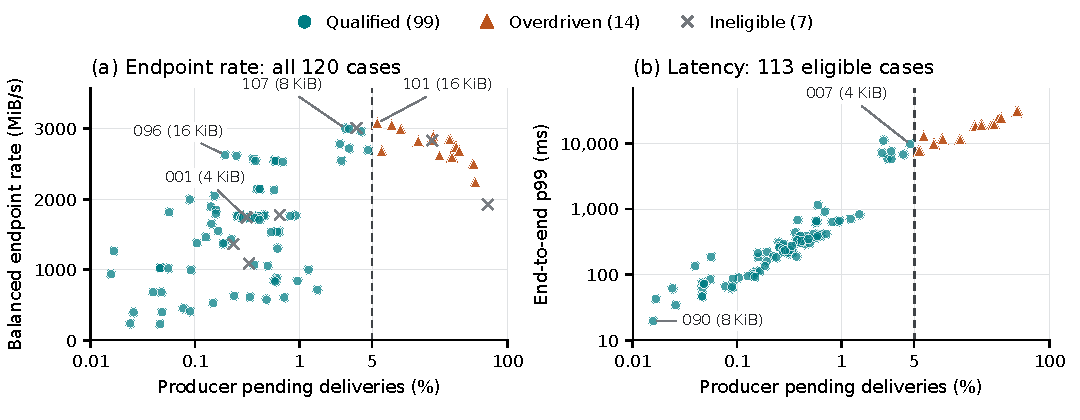
\includegraphics[width=\linewidth]{figures/kafka_operating_limits.pdf}
\caption{Kafka screening results. (a) All 120 observations: balanced endpoint rate against
producer pending-delivery ratio. (b) The 113 eligible observations: p99 latency
against the same ratio; seven invalid latency observations are omitted. The dashed
line marks the 5\% policy limit. Selected labels give configuration ID and
payload size. Every point is one run; both horizontal axes and the latency axis
are logarithmic. All pending ratios are positive (minimum 0.0157\%); no zeros
are omitted or clipped.}
\label{fig:kafka-operating-limits}
\end{figure}

The baseline, \texttt{cfg\_001}, achieves 1,767.1~MiB/s with 269~ms p99 and
0.296\% pending deliveries. The largest observed rate is 3,080.0~MiB/s from
\texttt{cfg\_101}, but its 5.599\% pending ratio exceeds the policy limit.
The highest qualified balanced endpoint rate is therefore \texttt{cfg\_107}:
3,001.5~MiB/s, 2.776\% pending deliveries, and 5,890~ms p99.
The rate gain comes with a substantially longer latency tail.

Byte rate, record rate, and latency favour different workloads.
With 1~KiB payloads, \texttt{cfg\_094} delivers the highest qualified record
rate, 1,023,762 records/s, at 999.8~MiB/s and 712~ms p99.
With 8~KiB payloads, \texttt{cfg\_090} has the lowest qualified p99,
19.5~ms, at 938.3~MiB/s. The 16~KiB workload \texttt{cfg\_096} combines
2,624.8~MiB/s with 221~ms p99, but delivers only 167,984 records/s.
A byte-rate ranking alone would hide these differences.

\subsection{Pending deliveries, latency, and overload}

All 14 eligible but overdriven screening cases exceed the 5\% pending-delivery
limit. Six also exceed the 10~s flush limit, and two exceed the 0.1\%
failed-send limit. The groups overlap: flush and failure counts do not represent
additional rejected cases. Qualified cases have a median pending ratio of
0.320\% and median p99 of 259~ms; the corresponding overdriven medians are
20.755\% and 19,000~ms. Thus a high endpoint rate can coexist with more unfinished producer work
at measurement end and long delivery delays.

The largest pending-delivery ratios occur among tested configurations combining
large payloads and high concurrency.
Among eligible 8~KiB cases with at least 104 total producer and consumer ranks,
only 2/7 qualify; median pending deliveries reach 19.29\% and p99 reaches
18.2~s. At 16~KiB and the same concurrency level, none of five cases qualify:
median pending deliveries are 32.00\% and p99 is 24.2~s, despite a median
2,743.0~MiB/s. At no more than 64 total ranks, all three eligible cases at
each of these payload sizes qualify, with median pending ratios below 0.1\%.
These are summaries of different configurations, not repeated estimates of
one setting.

Flush exposes the work left after production stops. The longest qualified
screening flush is 2.929~s; overdriven flushes range from 2.836 to 25.126~s.
All 99 qualified cases have zero failed sends, whereas the largest
failed-send percentage among eligible cases is 0.489\%. Passing record checks
after drain does not establish that consumers kept pace during measurement.

\begin{table}[H]
\centering
\footnotesize
\setlength{\tabcolsep}{6pt}
\begin{tabular}{@{}l l r r l r@{}}
\toprule
Varied limit & Tested values & Qualified & Overdriven & Highest qualified & MiB/s \\
\midrule
Pending (\%) & 2 & 92 & 21 & \texttt{cfg\_096} & 2,624.8 \\
 & 5 & 99 & 14 & \texttt{cfg\_107} & 3,001.5 \\
 & 10 & 103 & 10 & \texttt{cfg\_101} & 3,080.0 \\
\midrule
Flush (s) & 1 & 92 & 21 & \texttt{cfg\_096} & 2,624.8 \\
 & 3, 5, 10, 30 & 99 & 14 & \texttt{cfg\_107} & 3,001.5 \\
\midrule
Failed sends (\%) & 0, 0.01, 0.1, 1 & 99 & 14 & \texttt{cfg\_107} & 3,001.5 \\
\bottomrule
\end{tabular}
\caption{Screening-policy sensitivity using the same 113 eligible observations.
One limit varies at a time; the others stay at 5\% pending, 10 s flush, and 0.1\%
failed sends. Grouped values each give the listed outcome. Rates are balanced
endpoint rates, rounded for display; selection uses unrounded values.}
\label{tab:kafka-backlog-sensitivity}
\end{table}


Table~\ref{tab:kafka-backlog-sensitivity} shows that changing the pending or flush
limit can change the leader. Tightening failed sends to zero has no effect because
all 99 qualified cases already have zero failures. These are policy checks on
fixed observations, not new operating conditions or universal capacity boundaries.
Even under the declared policy, qualified p99 values reach 11.1 s because it
contains no application latency objective.

\subsection{Single-run parameter contrasts}

With 64 producer ranks instead of the baseline's 40, \texttt{cfg\_007} records
2,698.7~MiB/s, a 52.7\% higher screening rate. Its p99 is 9,810~ms
versus 269~ms, and pending deliveries are 4.571\% versus 0.296\%.
With only payload size changed from 4 to 8~KiB, the balanced endpoint rate is 2,546.8~MiB/s
(+44.1\%) and p99 is 11,100~ms. At 16~KiB, the corresponding one-factor
case \texttt{cfg\_030} is overdriven, with 22.151\% pending deliveries and
19,100~ms p99. More bytes per record eventually produce little additional
byte rate while delivery pressure continues to grow.

Smaller qualified rate increases occur with 80~ms producer linger
(+4.8\%, 185~ms p99) and 60 partitions (+2.6\%, 188~ms p99).
No tested one-factor alternative for consumer ranks, producer batch size,
either producer queue limit, or the consumer fetch settings exceeds the
baseline's qualified balanced endpoint rate. Across all 113 eligible cases, producer
ranks also correlate with pending deliveries and p99 (Spearman
$\rho=0.756$ and $0.759$). The mixed design and single-run contrasts identify
follow-up priorities; they do not establish statistical improvements or isolate
a physical bottleneck.

\subsection{Repeated validation and broker-profile selection}
\label{sec:profile-selection}

A three-pair instrumentation pilot on \texttt{cfg\_074} (16 producer ranks,
64 consumer ranks, 2~KiB records) compares timestamp sampling disabled with
sampling every tenth record.  The median paired endpoint-rate loss is 0.41\%,
below the 3\% pilot gate.  Each paired loss is $100(R_{\mathrm{off}}-R_{\mathrm{on}})/R_{\mathrm{off}}$
percent, where $R$ denotes balanced endpoint rate.  Disabled cases use the pilot's
separate validity rule.  This measures incremental latency-instrumentation cost for one
workload, not total benchmark overhead or overhead at the highest tested rates.

V1 executes ten shortlisted configurations in five randomized blocks.
All 50 observations are eligible, but only 27 qualify. Ranking qualified-observation
count before balanced endpoint rate selects the baseline: 5/5 qualified observations, median
1,746.4~MiB/s, and IQR 1.5~MiB/s. Both the screening byte-rate leader
\texttt{cfg\_107} and the producer-rank candidate \texttt{cfg\_007} qualify
in only 2/5 V1 observations. A promising screening point therefore does not suffice
for a recommendation.

Broker-profile tuning compares B0--B5 (Appendix Table~\ref{tab:broker-profiles}).
Each profile is screened once on four maximum-load anchors
(\texttt{cfg\_107}, \texttt{cfg\_061}, \texttt{cfg\_094}, and \texttt{cfg\_101})
and one fixed-rate latency anchor.  B0, B3, and B5 then receive two additional
runs per anchor.  The decision uses the resulting three-run medians, including
eligible overdriven runs.  B1, B2, and B4 are not advanced to confirmation.


The latency anchor uses a fixed aggregate target of 285,371 records/s,
set to 80\% of the median rate from three calibration runs. Its client settings
are given in Appendix~\ref{app:broker-settings}.

Profile eligibility additionally requires verified profile identity and hash,
process and required JMX samples, and tmpfs occupancy at most 75\%.
These profile-analysis checks extend the application validity checks with
diagnostic completeness and resource limits. The implementation combines them
in one \texttt{eligible} flag: a case can therefore fail profile comparison
because diagnostics are missing even when its application measurements are valid.
For each direction, the \texttt{iperf3} gate requires a completed record with a
parseable, finite, positive \texttt{megabytes\_per\_second} value. It tests neither
stability nor a minimum capacity. Changing a positive value alone cannot change
profile selection; a missing or nonpositive value can make a case ineligible.
The magnitudes enter diagnostic ratios only. Because the probe discrepancy
remains unresolved (Section~\ref{sec:kafka-resources}), we treat them as
unvalidated diagnostic metadata, not measured path-capacity bounds.
Acceptance requires at least a 3\% geometric-mean balanced endpoint-rate gain across the
four maximum-load anchors, no more than a 10\% fixed-load p99 increase, no
reduction in qualified counts on \texttt{cfg\_107} and \texttt{cfg\_061},
complete valid evidence, and no correctness or failed-send regression.
The final sampled request and response queues must also be empty; this is a
measurement-window check, not a post-drain observation.
Neither confirmed candidate passes: B3 and B5 achieve endpoint-rate ratios of
1.0161 and 1.0157 relative to B0, below the required 1.03. Their observed
fixed-load p99 median ratios are lower, at about 0.596 and 0.597. B0 is retained.
The rate-gain denominator is the matching B0 median for each of the four
maximum-load anchors; the geometric mean gives each anchor equal weight.
The latency anchor is excluded from that mean. The supplement lists all
per-anchor medians, ratios, eligible counts, and qualified counts.

Final V2 validation again runs ten workloads in five randomized blocks,
now under frozen B0. All 50 observations are eligible and 41 qualify.
Table~\ref{tab:kafka-final} reports all ten workloads, ordered first by
qualified-observation count and then by median balanced endpoint rate; the remaining tie-breaks
are rate IQR, pending deliveries, flush, failed sends, and ID.
Medians and IQRs include all five eligible observations, including overdriven ones.

\begin{table}[H]
\centering
\small
\setlength{\tabcolsep}{5pt}
\begin{tabular}{@{}l c r r r r r@{}}
\toprule
Configuration & Q/5 & Median MiB/s & IQR & p99 ms & Pending \% & Flush s \\
\midrule
\texttt{cfg\_007} & 5/5 & 2,927.1 & 4.8 & 2,560 & 1.237 & 0.480 \\
\texttt{cfg\_062} & 5/5 & 2,842.1 & 99.4 & 6,510 & 1.870 & 1.449 \\
\texttt{cfg\_049} & 5/5 & 2,795.5 & 56.5 & 6,340 & 3.375 & 1.897 \\
\texttt{cfg\_096} & 5/5 & 2,622.5 & 27.2 & 270 & 0.170 & 0.076 \\
\texttt{cfg\_001} & 5/5 & 1,745.5 & 17.2 & 224 & 0.307 & 0.100 \\
\texttt{cfg\_094} & 5/5 & 1,002.2 & 3.0 & 756 & 1.146 & 0.391 \\
\texttt{cfg\_113} & 4/5 & 3,009.2 & 87.8 & 6,760 & 4.085 & 1.800 \\
\texttt{cfg\_107} & 4/5 & 3,001.7 & 151.7 & 7,620 & 3.982 & 2.086 \\
\texttt{cfg\_061} & 3/5 & 2,946.3 & 82.2 & 7,950 & 4.768 & 2.575 \\
\texttt{cfg\_101} & 0/5 & 2,868.3 & 171.3 & 11,400 & 10.454 & 5.450 \\
\bottomrule
\end{tabular}
\caption{Final Kafka validation under frozen B0. Q/5 counts qualified observations;
all five observations per configuration are eligible. Rate medians and IQRs refer to
the balanced endpoint rate in MiB/s;
p99, producer pending-delivery ratio, and flush are medians across observations. Median
failed-send percentages are zero throughout. Qualification is assessed per
observation, rather than from the medians. Endpoint minima and classifications
were recomputed from retained rows; p99 values come from retained per-run summaries.
Displayed decimals do not imply measurement accuracy.}
\label{tab:kafka-final}
\end{table}


Within V2, the ranking places \texttt{cfg\_007} first: 64 producer and
40 consumer ranks with the other baseline settings unchanged. It qualifies in
5/5 observations and delivers median 2,927.1~MiB/s (749,340 records/s), with
IQR 4.8~MiB/s, 1.237\% pending deliveries, and 0.480~s flush.
None of its observations has failed sends. The faster medians of
\texttt{cfg\_113} and \texttt{cfg\_107} do not outrank it: each has one
overdriven observation, which their median operational metrics would conceal.
\texttt{cfg\_101} qualifies in none of five observations, with median pending
deliveries of 10.454\%.

This selection describes the retained V2 observations under the stated policy. The selected
workload's median p99 is 2,560~ms, versus 224~ms for the baseline.
The 5/5-qualified \texttt{cfg\_096} offers 2,622.5~MiB/s at 270~ms p99,
but its 16~KiB payload reduces the balanced record rate to 167,838 records/s.
For balanced record rate, \texttt{cfg\_094} reaches 1,026,286 records/s with
1~KiB payloads and 5/5 qualification. Applications requiring lower latency
would need to include that limit in their selection policy.

V1 and V2 are separate campaign stages. The change from the V1 baseline
leader to the V2 \texttt{cfg\_007} leader cannot be attributed to broker-profile
tuning, because B0 was retained. The datasets do not isolate a single cause
for the difference between stages.  The V2 ranking therefore does not establish
a stable recommendation across campaigns.

Using only qualified observations for the secondary rate median leaves the
V2 order unchanged. In V1, \texttt{cfg\_061} moves from ninth to sixth,
\texttt{cfg\_107} from eighth to seventh, \texttt{cfg\_007} from sixth to eighth,
and \texttt{cfg\_049} from seventh to ninth; both stage leaders are unchanged.
This sensitivity check changes only the rate median, retaining qualified counts
and subsequent tie-breaks. A zero-qualified case has no such median and remains
behind cases with positive qualified counts. Full ranks and medians are in the
companion supplement.

Figure~\ref{fig:validation-blocks} shows that variation also occurs within V1.
Only 3/10 workloads qualify in each of its first three blocks, compared with
9/10 in each of the last two.  This shift coincides with the batch-allocation
boundary: blocks 1--3 share one allocation and blocks 4--5 another.
For \texttt{cfg\_007}, the V1 pending-delivery ratio falls from
12.642--14.695\% in the first batch to 3.815\% and 1.360\% in the second.
V2 also spans two batches; its block counts are 9, 9, 8, 7, and 8.
Thus five blocks are not five independent allocation-level repetitions.
The association with batch boundaries warrants investigation but does not
identify a hardware, network, or software cause.

\begin{figure}[!htbp]
\centering
\resizebox{0.97\linewidth}{!}{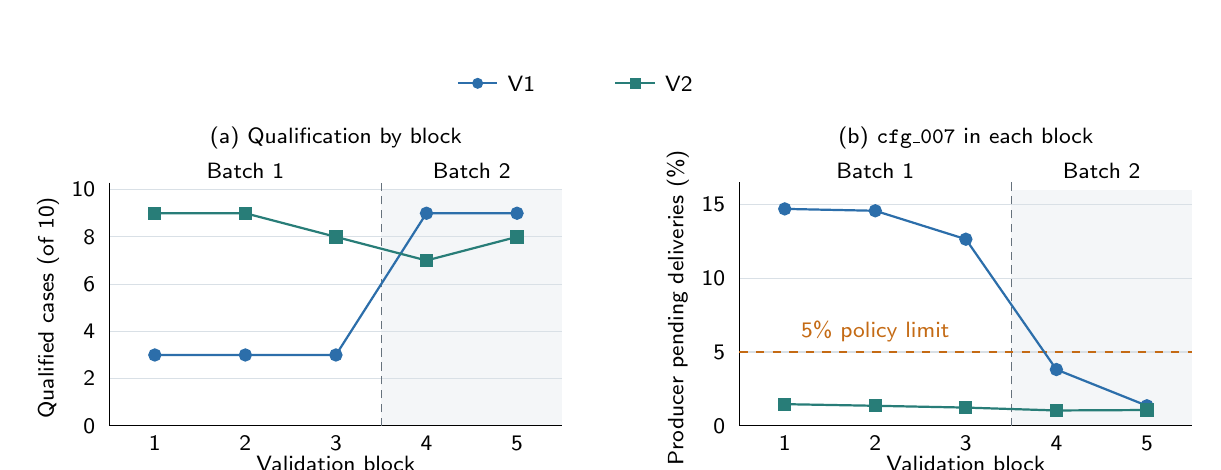
\begin{tikzpicture}[font=\sffamily\footnotesize]
\draw[mqblue,thick] (5.0,4.35) -- (5.5,4.35)
 node[right,text=black] {V1};
\fill[mqblue] (5.25,4.35) circle (2pt);
\draw[mqteal,thick] (7.0,4.35) -- (7.5,4.35)
 node[right,text=black] {V2};
\fill[mqteal] (7.18,4.28) rectangle (7.32,4.42);
\begin{scope}[x=1.15cm,y=0.30cm]
\fill[mqgrid!30] (3.5,0) rectangle (5.5,10);
\foreach \y in {0,2,4,6,8,10} {
 \draw[mqgrid] (0.5,\y) -- (5.5,\y);
 \node[left] at (0.45,\y) {\y};
}
\draw (0.5,10.3) -- (0.5,0) -- (5.5,0);
\draw[densely dashed,mqgray] (3.5,0) -- (3.5,10.3);
\foreach \x in {1,...,5} \node[below] at (\x,0) {\x};
\node[rotate=90] at (-0.18,5) {Qualified cases (of 10)};
\node at (3,-1.6) {Validation block};
\node at (2,10.8) {Batch 1};
\node at (4.5,10.8) {Batch 2};
\node at (3,12.2) {(a) Qualification by block};
% Verified from the ten case rows per block.
\draw[mqblue,thick] plot[mark=*,mark size=2pt] coordinates
 {(1,3) (2,3) (3,3) (4,9) (5,9)};
\draw[mqteal,thick] plot[mark=square*,mark size=2pt] coordinates
 {(1,9) (2,9) (3,8) (4,7) (5,8)};
\end{scope}
\begin{scope}[xshift=8cm,x=1.15cm,y=0.1875cm]
\fill[mqgrid!30] (3.5,0) rectangle (5.5,16);
\foreach \y in {0,5,10,15} {
 \draw[mqgrid] (0.5,\y) -- (5.5,\y);
 \node[left] at (0.45,\y) {\y};
}
\draw (0.5,16.5) -- (0.5,0) -- (5.5,0);
\draw[densely dashed,mqgray] (3.5,0) -- (3.5,16.5);
\draw[dashed,mqorange,thick] (0.5,5) -- (5.5,5);
\node[above,text=mqorange] at (2,5) {5\% policy limit};
\foreach \x in {1,...,5} \node[below] at (\x,0) {\x};
\node[rotate=90] at (-0.18,8) {Producer pending deliveries (\%)};
\node at (3,-2.56) {Validation block};
\node at (2,17.28) {Batch 1};
\node at (4.5,17.28) {Batch 2};
\node at (3,19.52) {(b) \texttt{cfg\_007} in each block};
% Verified from the cfg_007 pending-delivery counts and send attempts.
\draw[mqblue,thick] plot[mark=*,mark size=2pt] coordinates
 {(1,14.695) (2,14.567) (3,12.642) (4,3.815) (5,1.360)};
\draw[mqteal,thick] plot[mark=square*,mark size=2pt] coordinates
 {(1,1.469) (2,1.359) (3,1.237) (4,1.042) (5,1.072)};
\end{scope}
\end{tikzpicture}}
\caption{Validation by block, recomputed from the retained case rows.
Each stage uses two batch allocations, separated by the vertical dashed line;
the V1 and V2 batches are distinct.  Panel (a) counts qualified workloads out
of ten; panel (b) shows one observation of \texttt{cfg\_007} per block.
The V1 change aligns with its allocation boundary, but this does not establish
an allocation effect.}
\label{fig:validation-blocks}
\end{figure}

\subsection{Resource use and bottleneck evidence}
\label{sec:kafka-resources}

We examined broker-process and JMX measurements for all 50 final validation
runs. Kafka documents separate metrics for request queues, request timing, and
handler idle time~\cite{kafkamonitoring}. Each process trace contributed 29--30 samples between the first
producer measurement-start timestamp and the last producer send-loop stop. All metrics required by the campaign resource checks were present. Table~\ref{tab:kafka-resources} summarizes six workloads
that represent the baseline, V2 leader, qualification boundary, overload,
low latency, and high record rate. JMX rates retain their smoothing windows:
byte rates use one-minute counter rates, handler idle uses a one-minute rate,
and GC uses 30-second rates. Selecting samples inside the application window
therefore does not make these instantaneous application-rate measurements.

\begin{table}[H]
\centering
\small
\setlength{\tabcolsep}{5pt}
\begin{tabular}{@{}lrrrrrr@{}}
\toprule
Config & CPU & Kafka in / out & Handler idle & Heap & GC & tmpfs max. \\
 & (\%) & (MiB/s) & (\%) & (GB) & (ms/s) & (\%) \\
\midrule
\texttt{cfg\_001} & 5.14 & 1,797 / 1,772 & 93.4 & 2.78 & 3.31 & 32.1 \\
\texttt{cfg\_007} & 4.21 & 2,959 / 2,946 & 95.3 & 2.80 & 3.71 & 53.0 \\
\texttt{cfg\_107} & 3.64 & 3,164 / 3,180 & 95.2 & 2.74 & 3.64 & 56.1 \\
\texttt{cfg\_101} & 3.80 & 3,139 / 3,132 & 95.2 & 2.63 & 3.51 & 56.2 \\
\texttt{cfg\_096} & 4.39 & 2,619 / 2,612 & 94.2 & 2.67 & 3.69 & 47.1 \\
\texttt{cfg\_094} & 5.17 & 1,034 / 1,037 & 93.3 & 2.73 & 3.32 & 19.3 \\
\bottomrule
\end{tabular}
\caption{Broker resources in final validation under B0. Entries are medians
across five runs of each run's monitoring-window mean, except tmpfs, which
is the maximum over all five runs. CPU is broker-process utilization divided
by the logical CPUs allowed to that process. Kafka byte rates are JMX rates converted to MiB/s;
heap uses decimal GB. GC is the mean exported collector time rate.
The baseline and \texttt{cfg\_007}, \texttt{cfg\_096}, and \texttt{cfg\_094}
qualified in 5/5 observations, \texttt{cfg\_107} in 4/5, and \texttt{cfg\_101} in 0/5.}
\label{tab:kafka-resources}
\end{table}


\paragraph{CPU and broker queues.}
For the V2 leader, \texttt{cfg\_007}, the median per-run mean broker CPU use
was 4.21\% of the capacity of the logical CPUs allowed to that process. This normalization
can conceal a busy thread or core; it does not measure client CPU or establish
unused capacity along the whole path. The strongest queue evidence is that
every final run had zero mean and zero 95th-percentile sampled request- and
response-queue sizes. Per-run mean request-handler idle ratios ranged from
92.3\% to 96.0\%. These observations do not show sustained accumulation in
the sampled broker request queues, although one-second sampling can miss
short bursts. Network-processor idle was outside the required metric set and unavailable;
request-handler idle cannot establish the state of Kafka's network threads.

The overloaded \texttt{cfg\_101} illustrates the distinction. Its median
producer pending ratio was 10.45\% and application p99 was 11.40~s, compared
with 1.24\% and 2.56~s for \texttt{cfg\_007}. Yet their median handler-idle
ratios were both about 95\%. Their request-queue timing summaries were
0.770 and 0.488~ms, respectively, and total broker-request timing summaries
were 4.755 and 4.264~ms. These JMX summaries average exported per-request-type
p99 values over the window before taking the median across observations; they
are not pooled request percentiles. They cannot be subtracted from
application p99 to locate a delay. Together with the empty sampled queues,
they nevertheless provide little evidence for sustained saturation of the
request-handler pool as the explanation for the seconds-long application
tails. Producer buffering, batching, callback progress, consumer polling,
and transport remain candidates; these data do not isolate one cause.
The producer pending ratio counts outstanding delivery callbacks, not Kafka
consumer-offset lag, so it cannot identify a consumer bottleneck by itself.

\paragraph{Memory and garbage collection.}
Across the 50 runs, mean heap use ranged from 2.43 to 3.14~GB. The largest
per-run 95th-percentile heap measurement was 5.26~GB, below B0's 8~GiB heap
limit. Reported mean GC time rates ranged from 3.22 to 4.04~ms/s.
The extraction averages the exported collector series, so this is not a
total JVM pause fraction or a maximum pause measurement. It provides no
sign of sustained GC pressure, but cannot exclude isolated pauses.
Maximum observed tmpfs occupancy was 56.46\%, below the campaign's 75\%
resource limit. Thus heap and log-space exhaustion are not supported by
these runs. Because logs used tmpfs, this experiment also gives no evidence
about persistent-disk write bottlenecks or memory-bandwidth saturation.

\paragraph{Traffic.}
For \texttt{cfg\_007}, median Kafka ingress and egress rates were
2,959 and 2,946~MiB/s, close to its 2,927~MiB/s application result. For
\texttt{cfg\_101}, the corresponding rates were 3,139 and 3,132~MiB/s while
the balanced endpoint rate was 2,868~MiB/s. These differences are not
packet-loss estimates: broker counters and application payload bytes have
different scopes, JMX rates are smoothed, and the producer rate includes flush time whereas
the consumer rate uses the measurement interval. The broker-node
\texttt{ib0} receive means were 3,057 and 3,272~MiB/s, respectively, but
include all interface traffic. Neither interface rates nor separate
preflight path tests provide a matched link-capacity denominator for these
concurrent flows.  Table~\ref{tab:network-probes} reports the retained
\texttt{iperf3} summaries.  There are two shared pairs, not 50 independent
network measurements.  Their roughly 10 Gbit/s TCP rates are lower than both
the documented 100 Gbit/s fabric rate and the observed aggregate Kafka byte
rates.  Missing raw probe and route records prevent resolving this discrepancy;
dividing Kafka rates by these probes would not measure link utilization.

\begin{table}[!htbp]
\centering
\footnotesize
\begin{tabular}{@{}lrrr@{}}
\toprule
Final-validation blocks & Case rows & Producer $\rightarrow$ broker & Broker $\rightarrow$ consumer \\
\midrule
1--3 & 30 & 10.134 & 9.968 \\
4--5 & 20 & 10.492 & 10.597 \\
\bottomrule
\end{tabular}
\caption{Retained pre-Kafka \texttt{iperf3} throughput in decimal Gbit/s.
The analysis stores decimal MB/s; conversion is MB/s $\times 8/1000$.
Each batch shares its directional pair across the listed case rows.}
\label{tab:network-probes}
\end{table}

These measurements identify workloads that exceed the declared producer-delivery
policy and exhibit long latency tails.  Locating a specific client, core, or
network bottleneck would require per-thread and client traces and matched
path measurements.



\section{Limitations}
\label{sec:threats}

The results describe this single-broker, RAM-backed deployment.  They do not
measure replicated storage, long-running retention, or failure recovery under
load.  No duration-sensitivity experiment establishes that the 15~s warm-up
and 30~s measurement reach steady state; slow changes may be missed. The fixed
source-ID sampling pattern may bias latency, which also excludes waiting before
submission and therefore
does not represent response time to an externally scheduled device arrival.  The single-run
screening contrasts show where to investigate; they do not establish causal
improvements.  Each five-block validation stage spans only two batch allocations,
so blocks do not independently sample hardware placement.  The observations
do not establish stability across campaigns or other hardware. Each block has
its own shuffled order, but reusing those orders in V2 does not independently
randomize positions across stages. Temporal effects within blocks may therefore
recur. Confirmation should use new orders across allocations and stages, or
balance configuration positions. Envelope checks do
not verify full payload contents, and aggregate delivery counts can conceal
offsetting losses and duplicates that per-consumer offset checks miss.

The retained campaign lacks its per-node hardware snapshot, actual CPU clocks
and binding, negotiated link rates, exact Kafka/client versions, and repository
commit.  Published partition and processor specifications in
Table~\ref{tab:system-hardware} do not recover those runtime observations. Some later analysis
files contain product-version labels, but these do not replace a campaign-time
version snapshot.  The versioned Kafka documentation cited here describes
metric semantics, not the version used in the campaign.  The current source
can be inspected and tested, but cannot be proven identical to the campaign
implementation.  The companion evidence supports checking the reported
summaries; missing raw per-rank evidence and campaign provenance prevent full
independent reconstruction. Section~\ref{sec:availability} identifies the
repository copy of the retained evidence; public access and immutable-release
protection for this copy have not yet been verified.

\section{Conclusion}
\label{sec:conclusion}

\system{} links Slurm experiment control, measurement checks, a declared
producer-delivery policy, and configuration ranking.  Its Kafka evaluation
shows why the largest byte rate alone is insufficient for selection.
Within the retained V2 stage under B0, \texttt{cfg\_007} ranks first with five
qualified observations, median balanced endpoint rate of 2,927~MiB/s, and
median p99 latency of 2.56~s. It qualifies in only two V1 observations, and V1
qualification changes at an allocation boundary. These short-window results
support auditing a stage-specific decision, not a stable Kafka recommendation.
Confirmation requires independent allocations, longer measurement windows,
complete runtime provenance, and matched network and consumer-progress traces;
the retained evidence identifies neither a unique bottleneck nor sustained capacity.


\section{Code and Evidence Availability}
\label{sec:availability}

The \system{} source code is hosted on GitHub~\cite{hpcmqbenchcode}:
\url{https://github.com/skysepehr/hpc-mqbench}. The
\href{https://github.com/skysepehr/hpc-mqbench/tree/kafka-paper-evidence-v1/Report/HPC_MQBench_Kafka_Evidence}{companion evidence folder}
contains the retained case rows, manifests, profile summaries, contracts,
verification scripts, and a table-to-input and figure-to-input guide. It
excludes the unavailable raw traces and campaign-time source snapshot.

\bibliographystyle{plainnat}
\begingroup
\footnotesize
\setlength{\bibsep}{2pt plus 0.2ex}
\bibliography{references}
\endgroup

\par\bigskip
\appendix
\section{Experimental Configuration}
\label{app:configuration}
\setcounter{table}{0}
\renewcommand{\thetable}{\thesection.\arabic{table}}

This appendix collects the configuration details for the Kafka evaluation.
Published hardware specifications are distinguished from retained campaign
settings and do not substitute for a campaign-time hardware inventory.

\subsection{System and runtime settings}

\begin{table}[!htbp]
\centering
\footnotesize
\begin{tabularx}{\linewidth}{@{}L{0.23\linewidth}Y@{}}
\toprule
Property & Published specification or retained setting \\
\midrule
Platform & GWDG Emmy Phase 3, \texttt{standard96s}; Rocky Linux 8~\cite{gwdgcpupartitions} \\
Processor per node & Two Intel Xeon Platinum 8468 (Sapphire Rapids) processors~\cite{gwdgcpupartitions} \\
CPU cores per node & $2\times48=96$ physical cores; the processor model supports two threads per core~\cite{gwdgcpupartitions,intel8468} \\
CPU frequency & 2.10 GHz base, up to 3.80 GHz maximum turbo (processor specifications, not measured run frequencies)~\cite{intel8468} \\
RAM per node & 514,000 MB as listed by GWDG; this is not a retained measurement of available memory~\cite{gwdgcpupartitions} \\
Network & 100 Gbit/s Omni-Path fabric~\cite{gwdgcpupartitions}; campaign traffic monitored on \texttt{ib0} \\
Allocation & Four exclusive nodes: producer/controller, broker, consumer, monitoring/results \\
Kafka log storage & RAM-backed \texttt{/dev/shm}; no persistent-disk throughput evaluated \\
\bottomrule
\end{tabularx}
\caption{System configuration. Hardware and OS entries are published partition
or processor specifications; allocation and log-storage settings come from the
campaign. The interface name \texttt{ib0} does not identify the physical fabric.}
\label{tab:system-hardware}
\end{table}

Recorded runtimes are Slurm 26.05.1, Python 3.11.9, Open MPI 5.0.6, and
OpenJDK 17.0.11. Exact campaign-time Kafka and client-library versions were not
retained. Each case uses a 15 s warm-up, a 30 s measurement interval, a 30 s
producer flush timeout, and a consumer drain of up to 60 s after flush.
Timestamp sampling is every tenth measurement record. The delivery policy
allows at most 5\% pending deliveries, 10 s flush, and 0.1\% failed sends;
Section~\ref{sec:measurement} defines their timing and accounting semantics.

\subsection{Workload baseline and screening levels}

\begin{table}[!htbp]
\centering
\footnotesize
\begin{tabularx}{\linewidth}{@{}L{0.28\linewidth}L{0.14\linewidth}Y@{}}
\toprule
Parameter & Baseline & Tested levels \\
\midrule
Producer MPI ranks & 40 & 16, 24, 32, 40, 48, 56, 64 \\
Consumer MPI ranks & 40 & 16, 24, 32, 40, 48, 56, 64 \\
Topic partitions & 120 & 60, 90, 120, 180, 240 \\
Producer batch size & 1 MiB & 256 KiB, 512 KiB, 1 MiB, 2 MiB, 4 MiB \\
Producer linger & 20 ms & 0, 5, 10, 20, 40, 80 ms \\
Payload size & 4 KiB & 1, 2, 4, 8, 16 KiB \\
Producer queue messages & 1,000,000 & 500,000; 1,000,000; 2,000,000 \\
Producer queue capacity & 1,024 MiB & 512, 1,024, 2,048 MiB \\
Consumer fetch minimum & 1 MiB & 256 KiB, 1 MiB, 2 MiB, 4 MiB, 8 MiB \\
Consumer fetch wait & 50 ms & 10, 25, 50, 100 ms \\
Consumer fetch maximum & 8 MiB & 4, 8, 16, 32 MiB \\
\bottomrule
\end{tabularx}

\caption{Screened Kafka settings.  The baseline is \texttt{cfg\_001}.
Client buffer, batching, and fetch settings apply per client.
MiB and KiB denote $2^{20}$ and $2^{10}$ bytes.}
\label{tab:parameter-space}
\end{table}

The baseline is \texttt{cfg\_001}; the V2-selected \texttt{cfg\_007} changes only
producer ranks from 40 to 64. The listed levels define the screened parameter
space, not a full factorial experiment. The 120-case design and shortlist
construction are described in Section~\ref{sec:experimental-setup}.

\clearpage
\subsection{Broker profiles and the latency anchor}
\label{app:broker-settings}

\begin{table}[H]
\centering
\small
\setlength{\tabcolsep}{9pt}
\begin{tabular}{@{}lrrrr@{}}
\toprule
Profile & Network threads & I/O threads & Heap (GiB) & Log segment (bytes) \\
\midrule
B0 & 8 & 16 & 8 & $2^{30}$ \\
B1 & 16 & 32 & 16 & $2^{30}$ \\
B2 & 32 & 64 & 32 & $2^{30}$ \\
B3 & 48 & 96 & 32 & $2^{30}$ \\
B4 & 48 & 96 & 64 & $2^{30}$ \\
B5 & 48 & 96 & 64 & $2^{31}-1$ \\
\bottomrule
\end{tabular}
\caption{Screened broker profiles. All use G1 garbage collection; B0 is retained
for final validation. Log segments are in bytes: $2^{30}$ is 1 GiB and
$2^{31}-1$ is 2 GiB minus one byte.}
\label{tab:broker-profiles}
\end{table}

B0 uses an 8 GiB heap, eight network threads, sixteen I/O threads, 1 MiB socket
buffers, and 1 GiB log segments. The deployment uses one KRaft broker,
replication factor one, \texttt{acks=1}, no compression, and RAM-backed logs.

The latency anchor uses the baseline's 40/40 ranks, 120 partitions, and 4~KiB
records, but a 32~KiB batch, 1~ms linger, 1-byte fetch minimum, and 1~ms fetch
wait.  Its aggregate target is 285,371 records/s, set to 80\% of the median
rate from three calibration runs.  Other client settings remain at baseline.

\end{document}
